\documentclass[12pt,a4paper]{ctexart}
\usepackage{geometry}
\geometry{left=2.5cm,right=2.5cm,top=2.0cm,bottom=2.5cm}
% \usepackage[english]{babel}
\usepackage{amsmath,amsthm}
\usepackage{amsfonts}
\usepackage[longend,ruled,linesnumbered]{algorithm2e}
\usepackage{fancyhdr}
\usepackage{array}
\usepackage{listings}
\usepackage{color}
\usepackage{graphicx}
\usepackage{minted}
\usepackage{float}
\usepackage[defaultmono]{droidsansmono}

\graphicspath{{pics/}}
\ctexset{today=small}
\definecolor{codebg}{rgb}{0.95,0.95,0.95}

\input{personal_info/info.tex}

\begin{document}
    \begin{titlepage}
        \heiti
        \vspace*{64pt}
        \begin{center}
            \fontsize{48pt}{0} 算法设计与分析\\
            \vspace*{36pt}
            \fontsize{48pt}{0}{实\quad 验\quad 报\quad 告}\\
            \vspace*{48pt}
            \LARGE(2021\~{}2022 学年度\qquad 第 3 学期)\\
            \vspace*{48pt}
        
            \LARGE 实验名称\ \ \underline{\makebox[200pt]{\ExamTitle}}\\
            \LARGE 实验地点\ \ \underline{\makebox[200pt]{\ExamAddr}}\\
            \LARGE 实验日期\ \ \underline{\makebox[200pt]{\today}}\\
            \LARGE 学生姓名\ \ \underline{\makebox[200pt]{\MyName}}\\
            \LARGE 学生学号\ \ \underline{\makebox[200pt]{\MySID}}\\
            \LARGE 指导教师\ \ \underline{\makebox[200pt]{\TeacherName}}\\
            \vspace*{48pt}
            
            \LARGE 东南大学\quad  计软智学院 \quad 制
        \end{center}
    \end{titlepage}

\title{
  {\heiti \textbf{实验五\ 贪心算法}
    \footnote{要求:1、分析题请用书面化语言给出详细分析过程。2、实验请统一使用ex0*-学号-姓名的命名格式,latex版本请附上源代码并打包提交。}
    }
}
\date{}

\maketitle

\section*{\bf \color{black}{一、实验目的及意义}}
\noindent
\begin{enumerate}
	\item[(1)]  掌握贪心算法的基本思想、求解问题的基本步骤;
	\item[(2)]  学会利用贪心算法解决实际问题。
\end{enumerate}

\vspace{5pt}

\section*{二、实验内容与结果}
\subsection*{题目1:判断子序列}
\paragraph{题目内容}
\subparagraph{题目描述}
\begin{itemize}
    \item 字符串的一个子序列是原始字符串删除一些(也可以不删除)字符而不改变剩余字符相对位置形成的新字符串。(例如,"$ace$"是"$abcde$"的一个子序列,而"$aec$"不是)。
    \item 给定字符串$s$和$t$ ,判断$t$是否为$s$的子序列。
\end{itemize}

\subparagraph{输入格式}
    \begin{itemize}
        \item 第一行输入字符串 $s$ ;
        \item 第二行输入字符串 $t$ 。
    \end{itemize}
\subparagraph{输出格式}
    \begin{itemize}
        \item 输出是否为子序列,$true$ 或 $false$ 。
    \end{itemize}

\subparagraph{输入输出样例}
如下表
    \begin{figure}[h]
        \centering
        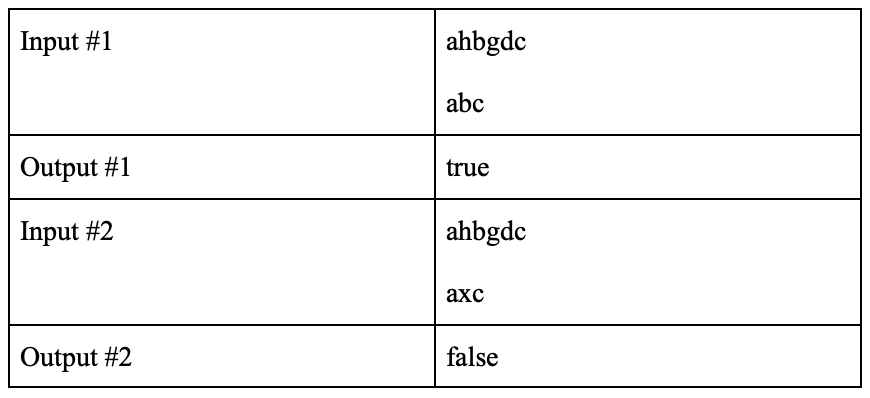
\includegraphics[width=0.80\textwidth]{q1_iodata.png}
    \end{figure}

\vspace{5pt}

\paragraph{实验环境}
\begin{itemize}
    \item 程序设计语言:C++
    \item 编程环境:
    \begin{itemize}
        \item 编辑器:Visual Studio Code (1.67.0)
        \item 编译器:g++ (GCC) 11.2.0
        \item 操作系统:ArchLinux 5.17.5-zen1-1-zen (64-bit)
    \end{itemize}
\end{itemize}

\vspace{5pt}

\paragraph{解答} 时间复杂度:$O(|s|)$($|s|$ 是字符串 $s$ 的长度)

源码:
\inputminted[bgcolor=codebg,frame=lines,autogobble,linenos=true,breaklines]{cpp}{src/t1.cpp}

\vspace{5pt}

\paragraph{实验结果}
(可附上截图)

\newpage

\subsection*{题目2:跳跃游戏}
\paragraph{题目内容}
\subparagraph{题目描述}
\begin{itemize}
    \item 给定一个非负整数数组,你最初位于数组的第一个位置。数组中的每个元素代表你在该位置可以跳跃的最大长度。你的目标是使用最少的跳跃次数到达数组的最后一个位置(假设你总是可以到达数组的最后一个位置)。
\end{itemize}

\subparagraph{输入格式}
    \begin{itemize}
        \item 第一行输入数组大小 $N$;
        \item 第二行输入数组。
    \end{itemize}

\subparagraph{输出格式}
    \begin{itemize}
        \item 输出最少跳跃次数。
    \end{itemize}
    
\subparagraph{输入输出样例}
如下表
    \begin{figure}[h]
        \centering
        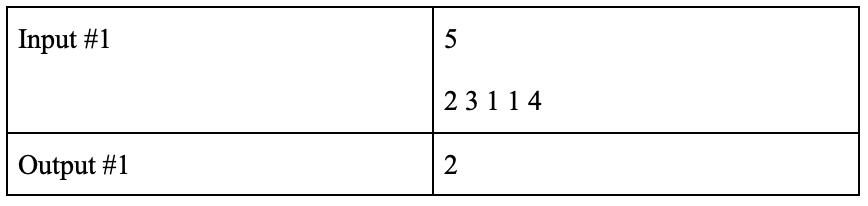
\includegraphics[width=0.80\textwidth]{q2_iodata.png}
    \end{figure}


\vspace{5pt}

\paragraph{实验环境}
\begin{itemize}
    \item 程序设计语言:C++
    \item 编程环境:
    \begin{itemize}
        \item 编辑器:Visual Studio Code (1.67.0)
        \item 编译器:g++ (GCC) 11.2.0
        \item 操作系统:ArchLinux 5.17.5-zen1-1-zen (64-bit)
    \end{itemize}
\end{itemize}

\vspace{5pt}

\paragraph{解答} 时间复杂度:$O(n)$

源码:
\inputminted[bgcolor=codebg,frame=lines,autogobble,linenos=true,breaklines]{cpp}{src/t2.cpp}

\vspace{5pt}

\paragraph{实验结果}
(可附上截图)

\newpage

\subsection*{题目3:最佳球迷}
\paragraph{题目内容}
\subparagraph{题目描述}

\begin{itemize}
    \item 作为球迷,一定想看尽量多的完整的比赛,当然,作为新时代的好青年,你一定还会看一些其它的节目,比如新闻联播(永远不要忘记关心国家大事)、觉醒年代、中国好声音,以及世界杯等等,假设你已经知道了所有你喜欢看的电视节目的转播时间表,你会合理安排吗?(目标是能看尽量多的完整节目)
\end{itemize}

\subparagraph{输入格式}
    \begin{itemize}
        \item 第一行输入一个整数 $N$ ,表示你想看的节目数;
        \item 后续输入第二行到第 $N$ 行,每行包括两个数据,表示该节目的开始和结束时间,为了简化问题,每个时间都用一个正整数表示。
    \end{itemize}

\subparagraph{输出格式}
    \begin{itemize}
        \item 输出能完整看到的电视节目的个数,每个测试实例的输出占一行。
    \end{itemize}
    

\subparagraph{输入输出样例}
如下表
    \begin{figure}[hp]
        \centering
        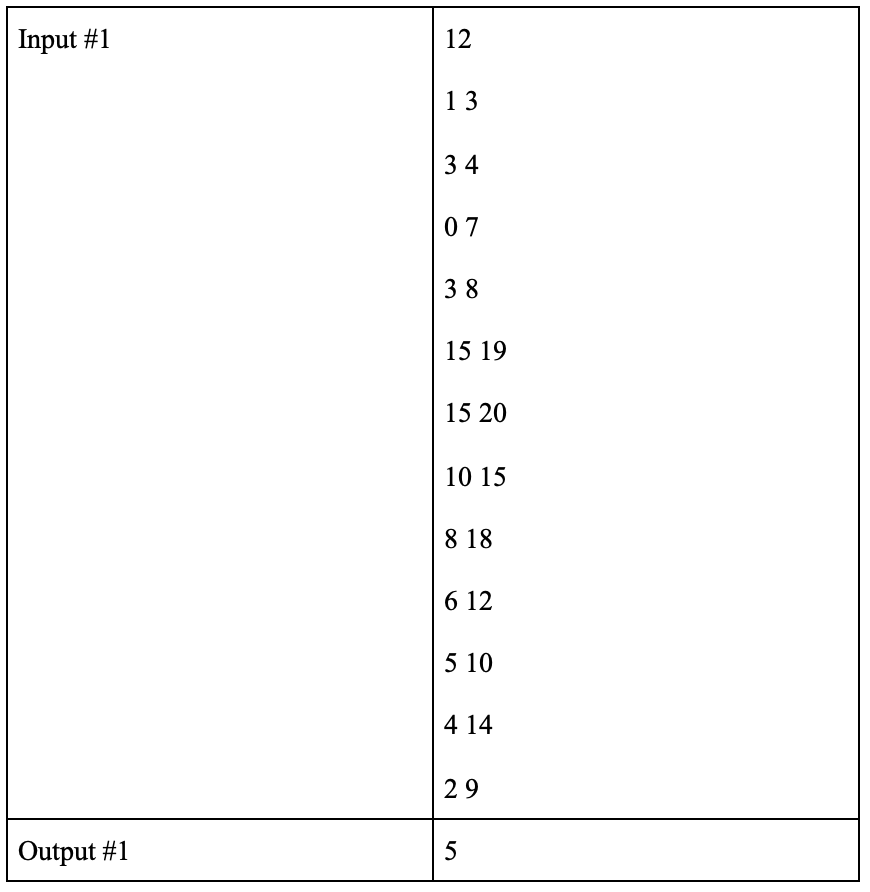
\includegraphics[width=0.80\textwidth]{q3_iodata.png}
    \end{figure}

\vspace{5pt}

\paragraph{实验环境}
\begin{itemize}
    \item 程序设计语言:C++
    \item 编程环境:
    \begin{itemize}
        \item 编辑器:Visual Studio Code (1.67.0)
        \item 编译器:g++ (GCC) 11.2.0
        \item 操作系统:ArchLinux 5.17.5-zen1-1-zen (64-bit)
    \end{itemize}
\end{itemize}

\newpage

\paragraph{解答} 时间复杂度:$O(N \log N)$

源码:
\inputminted[bgcolor=codebg,frame=lines,autogobble,linenos=true,breaklines]{cpp}{src/t3.cpp}

\vspace{5pt}

\paragraph{实验结果}
(可附上截图)

\newpage

\vspace{5pt}

\section*{三、心得体会}
    可根据“实验思考”部分作答,也可以根据个人具体体会作答。自己算法的创新点可在此处进行介绍,酌情加分。

\end{document} 
